\documentclass{article}

\usepackage{url} 

\usepackage[utf8]{inputenc}

\usepackage{pdfpages}
\usepackage{lastpage}
\usepackage{fancyhdr}
\usepackage{ngerman}
\usepackage{listings}

\usepackage{tabularx}
\usepackage{floatrow}
\usepackage[tableposition=top]{caption}
\floatsetup[table]{capposition=top}

\usepackage{amsmath, amssymb}

\usepackage[utf8]{inputenc}

\usepackage{xifthen}
\usepackage[numbib]{tocbibind}



\newcommand\twodigits[1]{%
   \ifnum#1<10 0#1\else #1\fi
}



\lhead{Spektralphotometer}
\rhead{20. November 2020\\T. Maier, J. Winkler}
%\cfoot{\twodigits{\thepage}~/ \pageref{LastPage}}
\cfoot{{\thepage}~/ \pageref{LastPage}}

\newcommand{\W}{\text{W}}
\newcommand{\V}{\text{V}}
\newcommand{\A}{\text{A}}


\newcommand{\mini}{\operatorname{min}}


\begin{document}

\parindent0cm

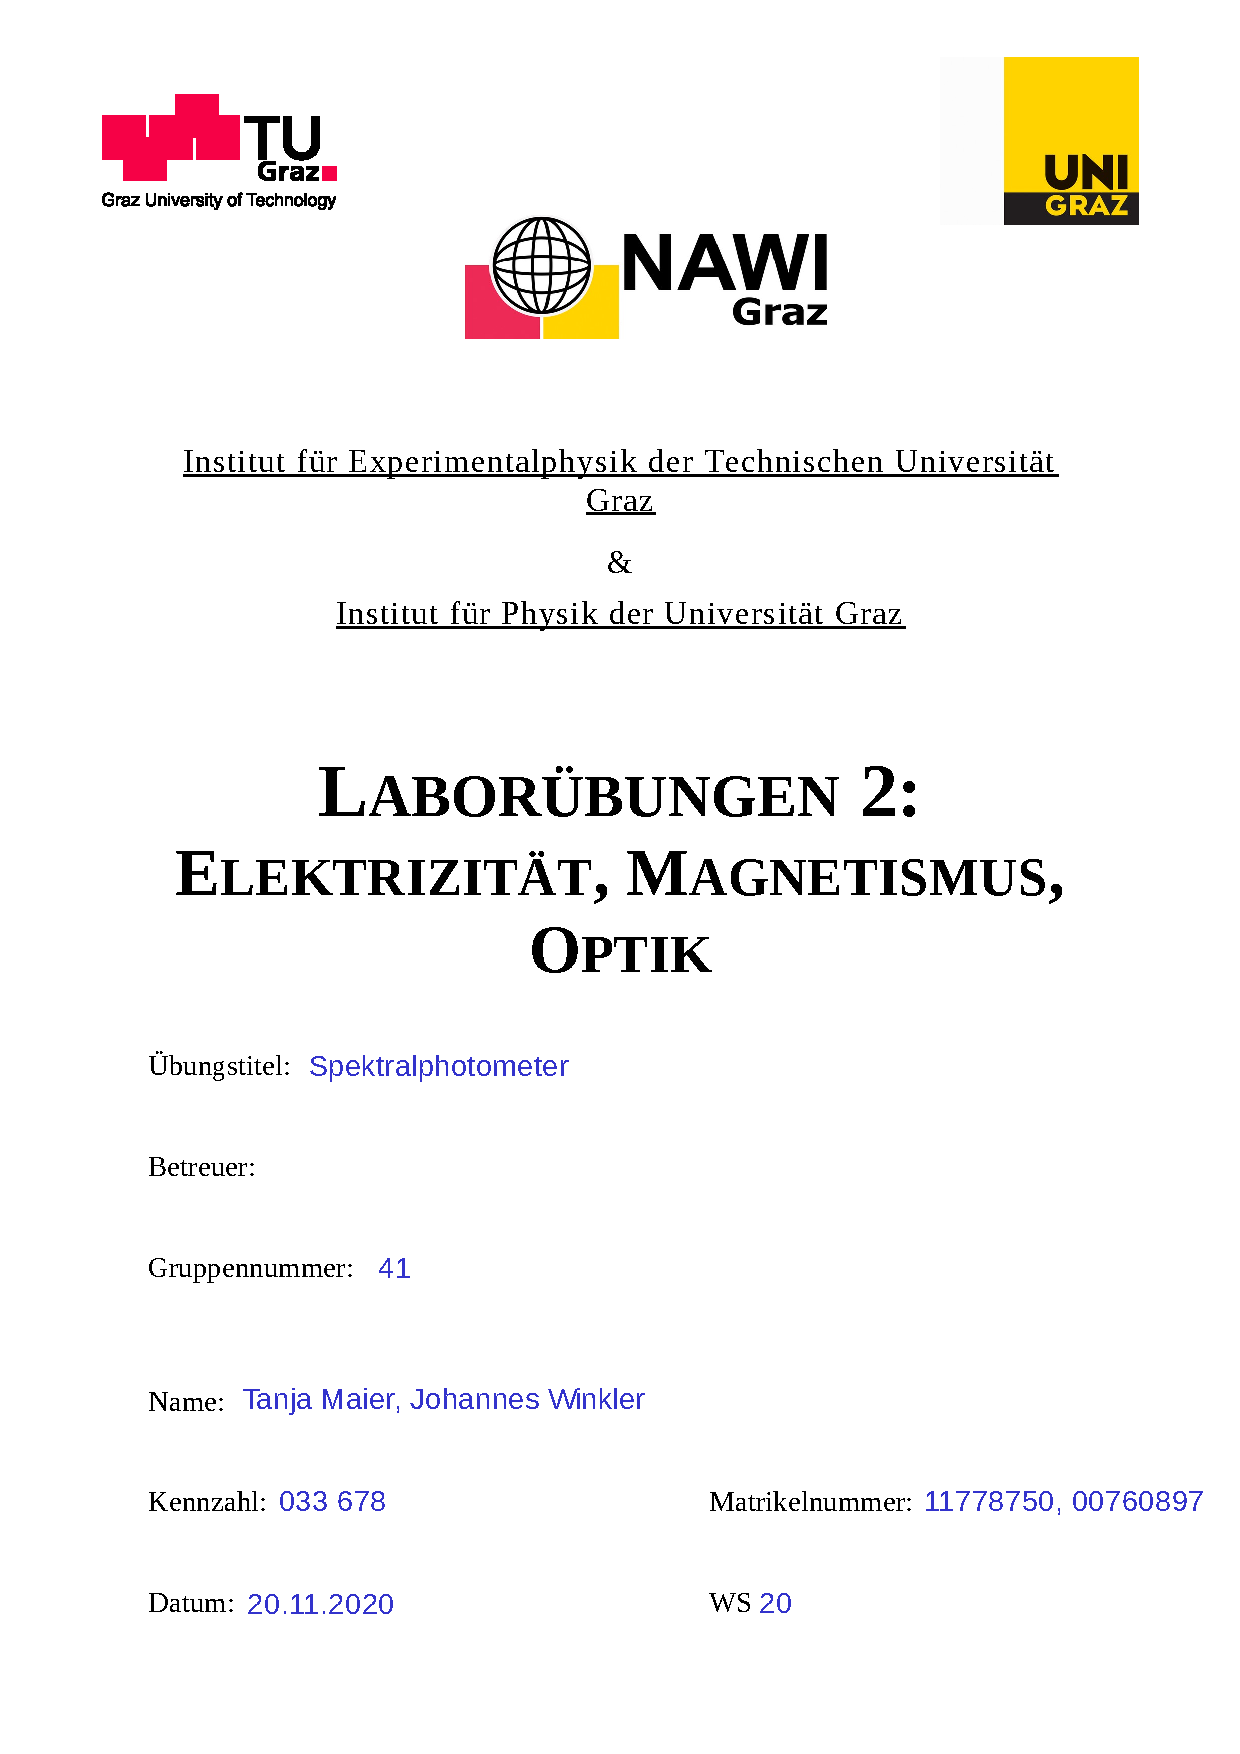
\includepdf{Deckblatt.pdf}


\pagestyle{fancy}

\tableofcontents
\newpage
\section{Aufgabenstellung}



\begin{enumerate}
\item Messen Sie mit dem Spektralphotometer die optische Transmission von Farbfiltern. Stellen Sie die Transmission und die (als logarithmisches Maß definierte) optische Extinktion als Funktion der Lichtwellenlänge dar. \item Zeigen Sie an zwei Farbfiltern die Additivität der Extinktion.
\item Bestimmen Sie die Stoffmengenkonzentration einer Methylenblaulösung. \item Diskutieren und erklären Sie anhand der gemessenen Spektren den Farbeindruck der jeweiligen Proben.
\item Messen Sie die Dicke einer Glasplatte durch Auswertung der Interferenzmaxima im Transmissionsspektrum
\end{enumerate}



\section{Voraussetzungen und Grundlagen}

\subsection{Transmission, Extinktion, Absorptionsquerschnitt}

Wenn Licht auf verschiedene Stoffe und Materialien scheint, kann es in unterschiedlichen Frequenzen oder Wellenlängen reflektiert, absorbiert und gestreut werden. Trifft Licht auf eine glatte Oberfläche oder einen homogenen Körper, so wird die Streuung Reflexion genannt. Beim Einfall auf eine teiltransparente Schicht ist das Verhältnis der transmittierten (als durch das Medium durchgelassenen) Intensität $I_T$ und der auf das Medium scheinende Lichtintensität $I_0$ gegeben durch
\begin{align}
\label{eq:trans}
T = \frac{I_T}{I_0}
\end{align}
wobei $T$ als Transmission bzw. Transmissionsgrad bezeichnet wird. Wichtig ist, dass $T < 1$ ist, da immer ein gewisser Teil des Lichts beim Kontakt mit dem Medium in eine andere Energieform (z.B. Wärme) umgewandelt (also absorbiert) oder einfach in andere Richtungen reflektiert (bzw. gestreut) wird.

Allerdings kann aus der Messung der transmittierten Intensität meist nicht auf jene Intensitätsanteile, die gestreut bzw. die absorbiert werden rückgeschlossen werden. Daher wird in der Spektroskopie oft das dekadisch logarithmische Maß der Lichtabschwächung (Extinktion) verwendet:

\begin{align}
\label{eq:ex}
E = -\log(T) = -\log\left(\frac{I_T}{I_0}\right) = \log\left(\frac{I_0}{I_T}\right)
\end{align}

Falls mehrere Extinktionsprozesse stattfinden, so können diese wegen der Gesetze für Logarithmen addiert werden. Außerdem können durch das logarithmische Maß Variationen von Lichtabschwächung über mehrere Größenordnungen übersichtlich dargestellt werden.

Die Lichtabschwächung bei einem homogenen Medium kann durch das Lambert-Beer'sche Gesetz beschrieben werden
\begin{align}
I_T(d) = I_0 \cdot \exp\left(-\alpha\cdot d\right)
\end{align}
wobei $d$ die Schichtdicke des Mediums und $\alpha$ der Extinktionskoeffizient ist.

Der Extinktionskoeffizient $\alpha$ hängt dabei vom molaren Extinktionskoeffizienten $\varepsilon_n$ und von der Stoffmengenkonzentration $c$ des gelösten Stoffes ab. Es gilt $\alpha = \varepsilon_n \cdot c$. Dadurch ergibt sich für das Lambert-Beer'sche Gesetz
\begin{align}
I_T(d) = I_0 \cdot \exp\left(-\varepsilon\cdot c\cdot d\right)
\end{align}

Dadurch kann die Extinktion mit $\varepsilon$ als dekadisch molarem Extinktionskoeffizienten $\varepsilon = \varepsilon_n / \operatorname{ln}(10)$ definiert werden als
\begin{align}
\label{eq:konzentration}
E = \log\left(\frac{I_0}{I_T}\right) = \varepsilon\cdot c\cdot d.
\end{align}

Der Beitrag eines einzelnen Moleküls zur Extinktion wirds als Absorptionsquerschnitt $q$ bezeichnet und definiert als
\begin{align}
q = \varepsilon\cdot \operatorname{ln}(10) / N_A
\end{align}
wobei $N_A$ die Avogadro-Konstante ist. Der Absorptionsquerschnitt kann jedoch (da er eine effektive Fläche angibt) erheblich vom geometrischen Molekülquerschnitt abweichen.


\subsection{Interferenzen an einer planparallelen Platte}


Wenn Weißlicht auf eine planparallele Platte trifft, so kommt es zur Interferenz. Das Interferenzmuster entsteht durch Auslöschen der Wellenlänge (destruktive Interferenz) oder Verstärkung der Wellenlängen (konstruktive Interferenz) und kann dabei sowohl einer Reflexion als auch einer Transmission entsprechen.

Der Gangunterschied $\Delta s$ ist  gegeben durch
\begin{align}
\label{eq:gangunterschied}
\Delta s  = 2\cdot n_p\cdot d = m\cdot\lambda_m
\end{align}
wobei $n_P$ die Brechzahl des Mediums und $d$ die Schichtdicke ist. Wenn der Gangunterschied einem ganzzahligen Vielfachen $m$ der Wellenlänge entspricht, so bildet sich ein Interferenzmaximum (konstruktive Interferenz). $\lambda_m$ sind die Wellenlängen, bei denen ein solches Maximum auftritt.

Die Wellenzahl $\nu = 1/\lambda$ ergibt daher
\begin{align}
v_m = \frac{m}{2\cdot n_p\cdot d}
\end{align}
Durch Auftragen der Wellenzahlen der Maxima als Funktion von m kann aus der Steigung der Geraden und der bekannten Brechzahl $n$ des Mediums die Schichtdicke $d$ ermittelt werden.


%\begin{figure}[H]
%\caption{Transformator}
%\label{fig:transformator}
%{\centering
%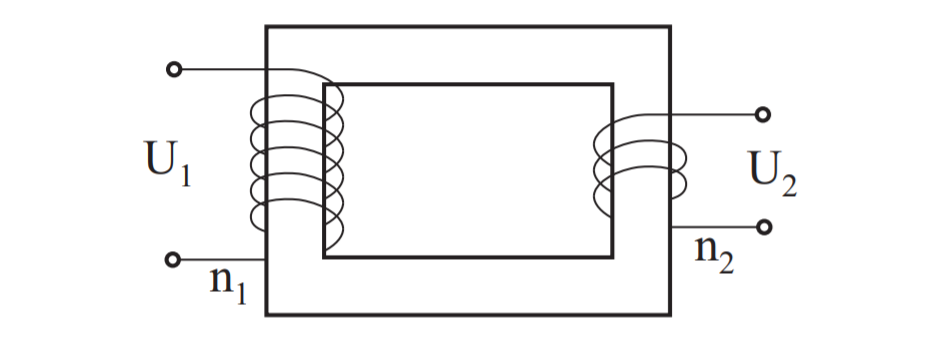
\includegraphics[scale=0.4]{transformator.png}
%~
%}
%\end{figure}



\section{Geräteliste}

\begin{table}[H]
\caption{Liste der verwendeten Geräte}

~

\begin{tabular}{l|p{3cm}p{3.5cm}llll}
Abk. & Gerätename    & Hersteller & Modell  \\
\hline
S & Spektralphotometer & THOR-Labs & CCS200/M \\
L & Lampe & THOR-Labs & QTH10/M \\
FR & Filter Rot & \\
FB & Filter Blau & \\
KW & Küvette mit Wasser &\\
KM & Küvette mit Methylenblau \\
GP & Glasplatten \\
PC & Computer mit Software SPLICCO
\end{tabular}
\end{table}

Sämtliche Daten wurden nach den Versuch mit Python3.8 ausgewertet, wobei für Grafiken die Library \texttt{Matplotlib} verwendet wird. 




\section{Beschreibung der Versuchsanordnung}

Der Versuchsaufbau ist in als Foto in Abbildung~\ref{fig:aufbau} dargestellt, in Abbildung~\ref{fig:aufbau2} ist der schematische Aufbau gezeigt.

\begin{figure}[H]
\caption{Versuchsaufbau, Arbeitsplatz 3.}
\label{fig:aufbau}
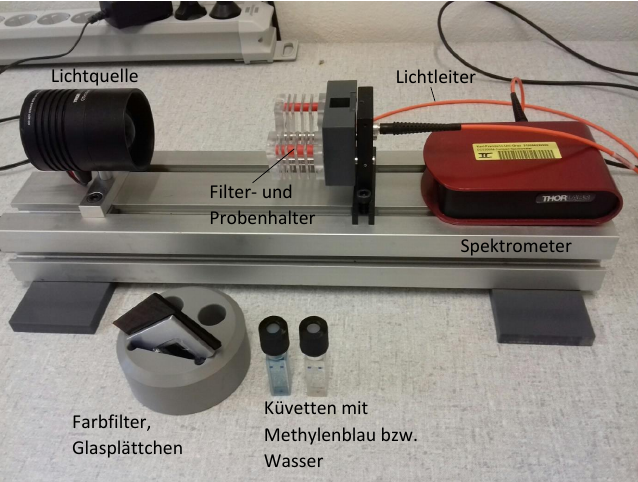
\includegraphics[scale=1.4]{aufbau.png}
\end{figure}


\begin{figure}[H]
\caption{Schematischer Aufbau des Versuchs. Gezeichnet mit Wacom Tablet im Programm Xournal.}
\label{fig:aufbau2}
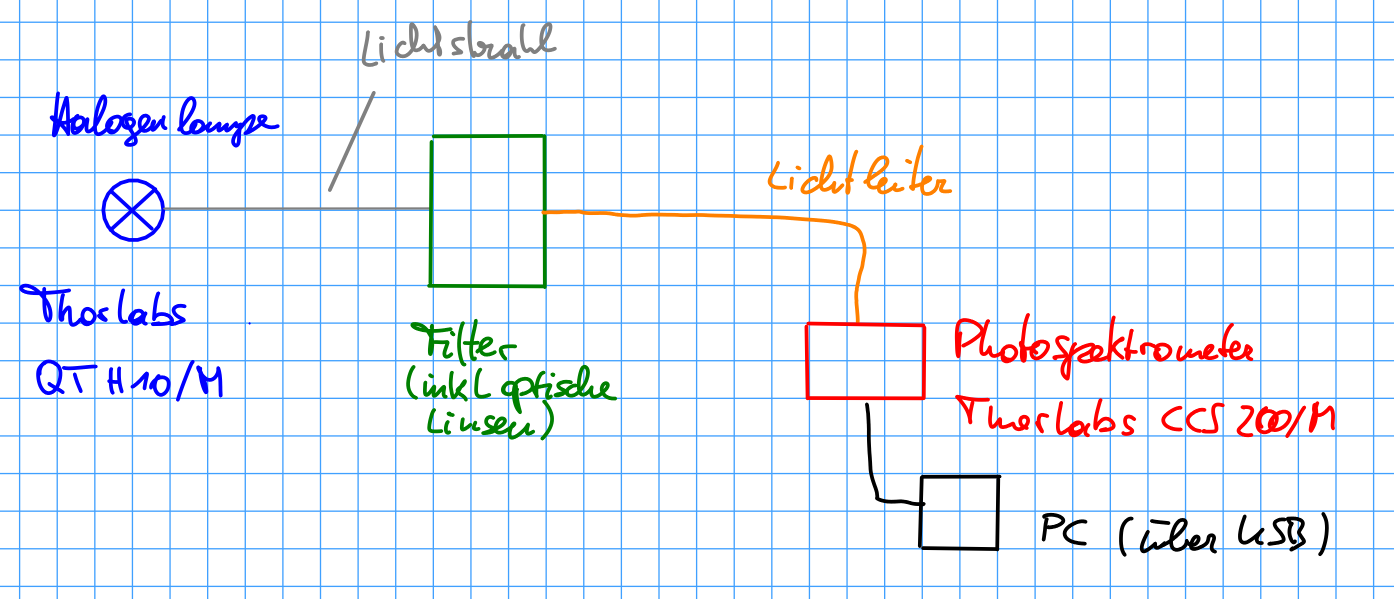
\includegraphics[scale=1.]{aufbau2.png}
\end{figure}

Formel~\eqref{eq:gangunterschied} wird durch Grafik~\ref{fig:aufbau3} veranschaulicht. Damit lässt sich aus den Interferenzmaxima der Rückschluss auf die Dicke einer Glasplatte ziehen. 

\begin{figure}[H]
\caption{Strahlengang bei Glasplatten. Gezeichnet mit Wacom Tablet im Programm Xournal.Gezeichnet mit Wacom Tablet im Programm Xournal.}
\label{fig:aufbau3}
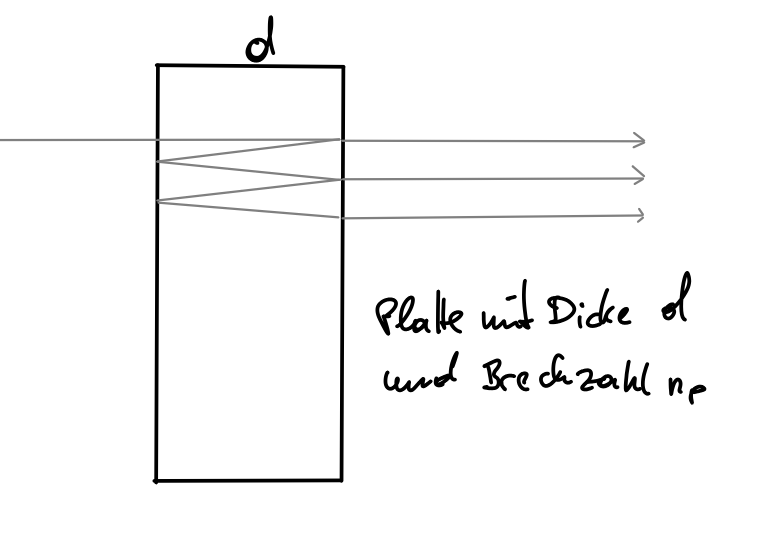
\includegraphics[scale=1.]{aufbau3.png}
\end{figure}


Das Spektralphotometer benutzt für die Zerlegung des Lichtes einen Czerny-Turner Monochromator, wie er in Abbildung~\ref{fig:monochromator} dargestellt ist. Das einfallende Licht A wird durch eine Blende gebündelt und gelangt dann auf einen Hohlspigel C. Von dort wird es zu einem Gitter D reflektiert, wo es in die Bestandteile gebrochen wird. Diese Bestandteile werden auf einen zweiten Hohlspiegel E reflektiert, danach werden diese durch eine verschiebbare Blende F selektiert und je nach Wellenlänge gemessen.

\begin{figure}[H]
\caption{Czerny-Turner Monochromator, (Quelle: \cite{monochromator}, Creative Commons by-sa 3.0 de)}
\label{fig:monochromator}
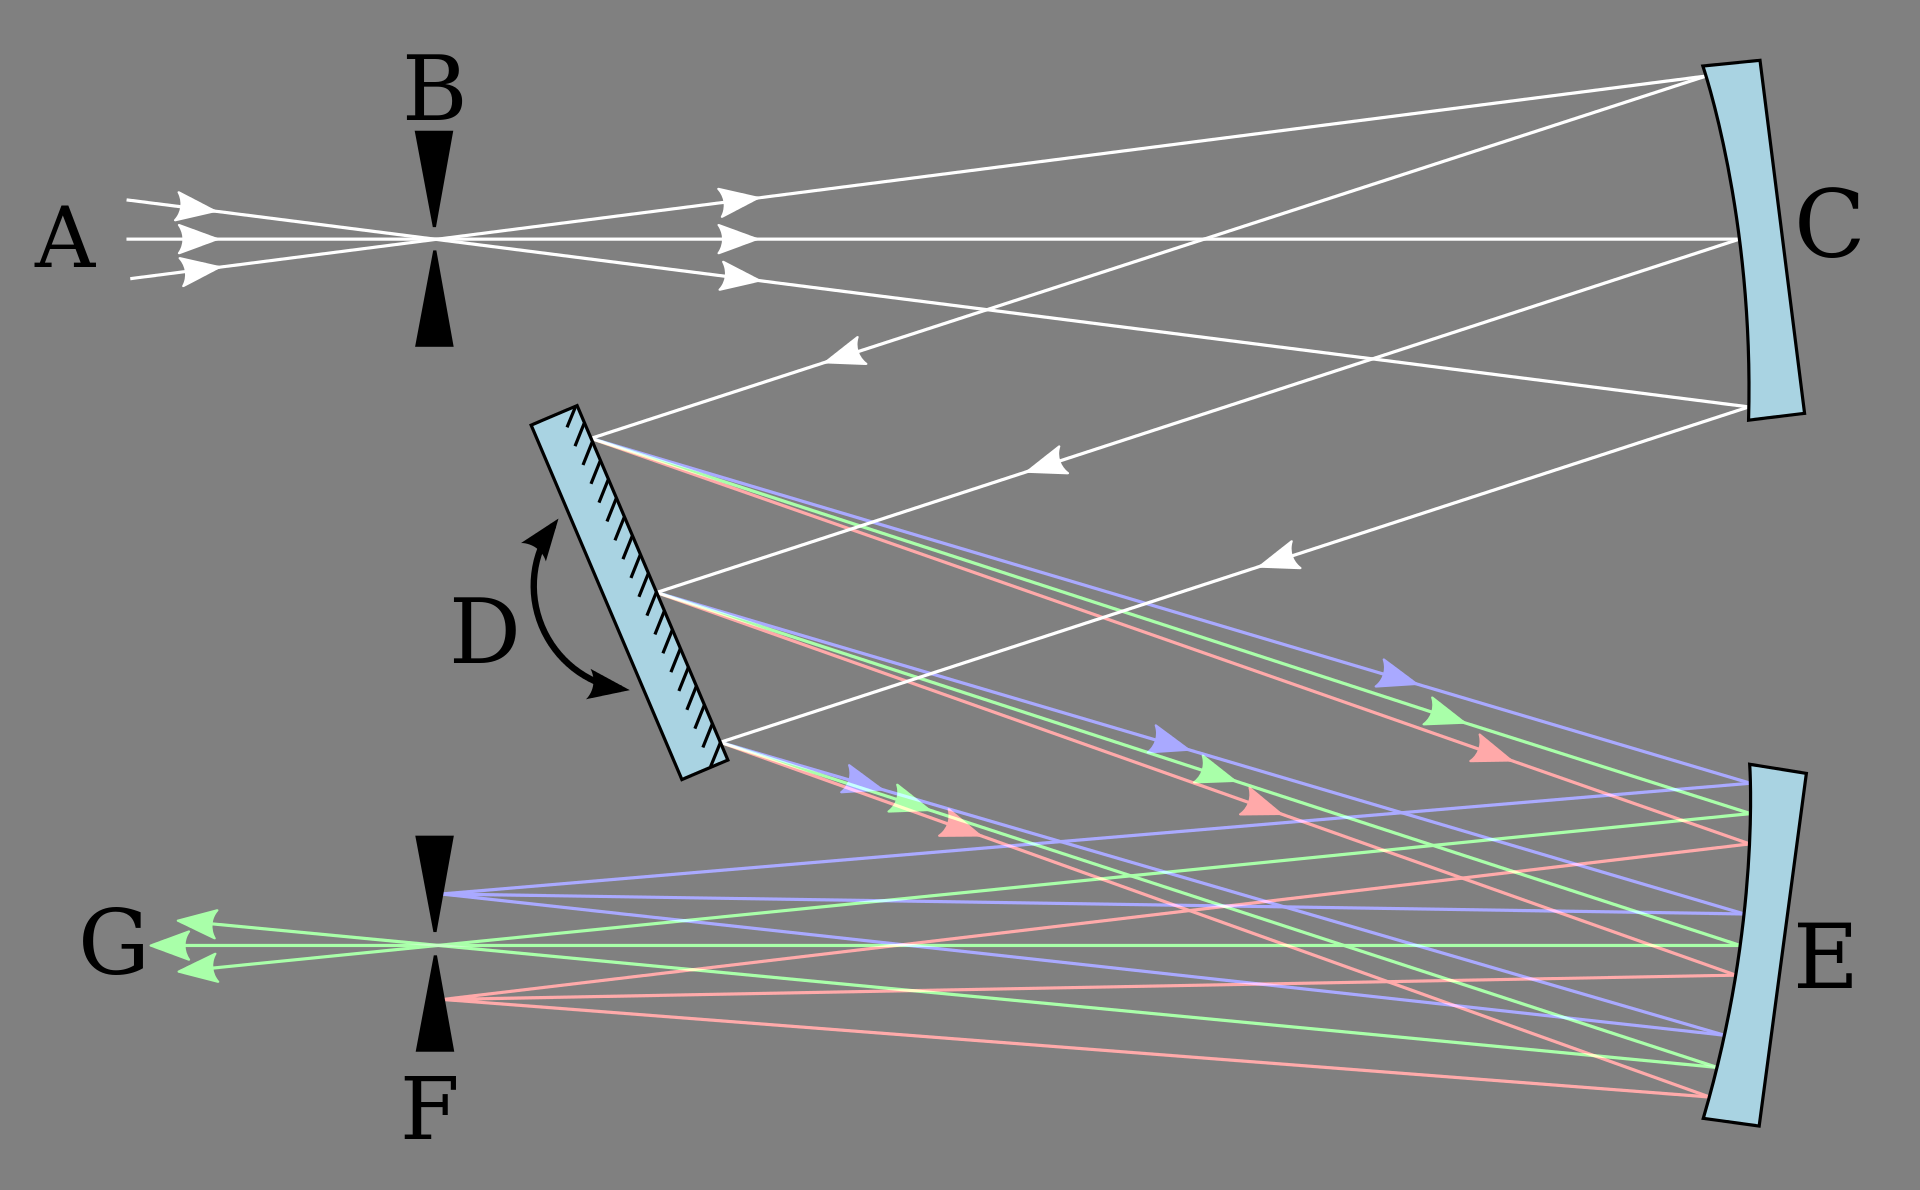
\includegraphics[scale=0.1]{monochromator.png}
\end{figure}


\section{Versuchsdurchführung und Messwerte}

Als erstes wurde die Halogen-Lampe eingeschalten und die Spektralphotometer-Software SPLICCO gestartet. In der Software wurde dann der Wellenlängenbereich auf $400-800$~nm eingestellt, die Integrationszeit (integration time) auf $0.9$~ms eingestellt, sodass das Spektrum der Lichtquelle über den gesamten angezeigten y-Achsenabschnitt gut skaliert wird. Die durchschnittlichen Aufnahmen (average scans) wurden auf 50 eingestellt.
Zur Korrektur der Hintergrundbeleuchtung musste die Halogen-Lampe wieder ausgeschalten werden und mit Save Background Correction gespeichert werden. So wird die Hintergrundbeleuchtung bei den folgenden Messungen automatisch abgezogen. Falls sich die Hintergrundbeleuchtung im Laufe des Experiments ändern sollte, so muss diese Korrektur wiederholt werden.

Bei allen Messungen der Intensität ist es vor der Messung nötig, dass ein Spektrum ohne Filter aufgenommen wird. Dieses wird als Referenzspektrum bezeichnet. Das Referenzspektrum ist nötig, um die Extinktion zu berechnen.

\subsection{Bestimmung der Transmission und der Extinktion für verschiedene Farbfilter}

Danach wurden die Intesitätsspektren für den roten und den blauen Farbfilter gemessen, insbesondere auch die Kombination dieser beiden. Die Intensitätsspektren sowie das Referenzspektrum liegen im csv Format vor.



Die gemessenen Intensitäten sind in Grafik \ref{fig:I_Methyl} zusammengefasst.

\begin{figure}[H]
\centering
\caption{Zusammenhang zwischen Intensität und Wellenlänge bei gegebenen Filter.}
\label{fig:I_Methyl}
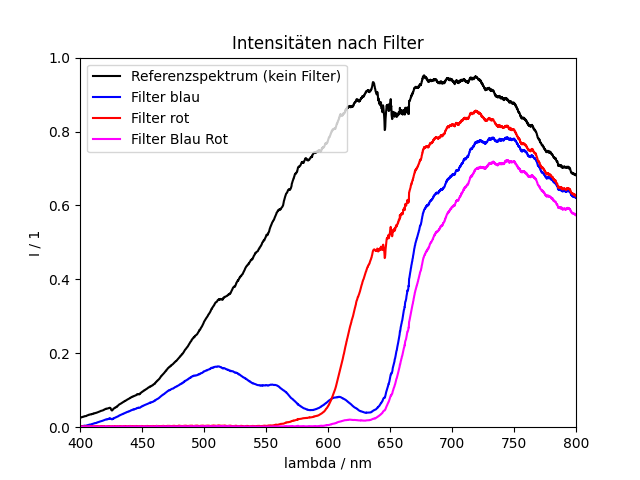
\includegraphics[scale=0.7]{FF_Intensitaeten.png}
\end{figure}





\subsection{Bestimmung der Stoffmengenkonzentration einer Methylenblaulösung}

Dafür wurde zuerst der Filterhalter gegen den Küvettenhalter ausgetauscht und die Küvette mit Wasser im Halter platziert und das Transmissionsspektrum von Wasser als Referenz gemessen. Dann wurde die Küvette mit Wasser gegen die Küvette mit Methylenblausäure ausgetauscht und ebenfalls das Transmissionsspektrum gemessen.



\begin{figure}[H]
\centering
\caption{Zusammenhang zwischen Intensität und Wellenlänge einmal bei einer Küvette mit Wasser (grau) als Referenzspektrum und einmal bei einer Küvette mit einer Lösung mit Methylenblau (Probe 1 aus der Angabe).}
\label{fig:I_methylenblau1}
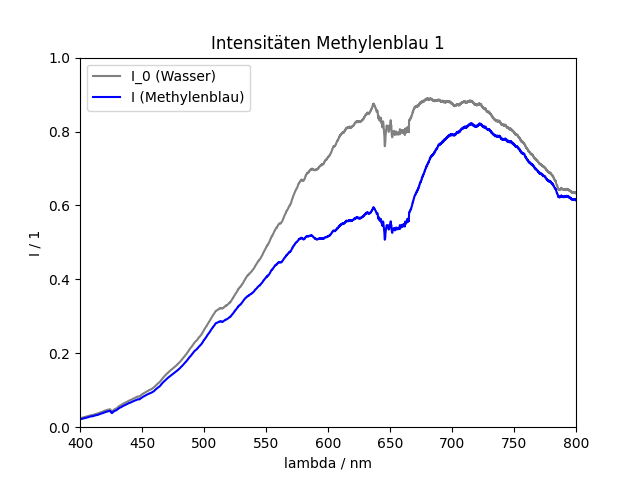
\includegraphics[scale=0.6]{MB_Intensitaeten_1.png}
\end{figure}

%\begin{figure}[H]
%\centering
%\caption{Zusammenhang zwischen Intensität und Wellenlänge einmal bei einer Küvette mit Wasser (grau) und einmal bei einer Küvette mit einer Lösung mit Methylenblau.}
%\label{fig:I_methylenblau2}
%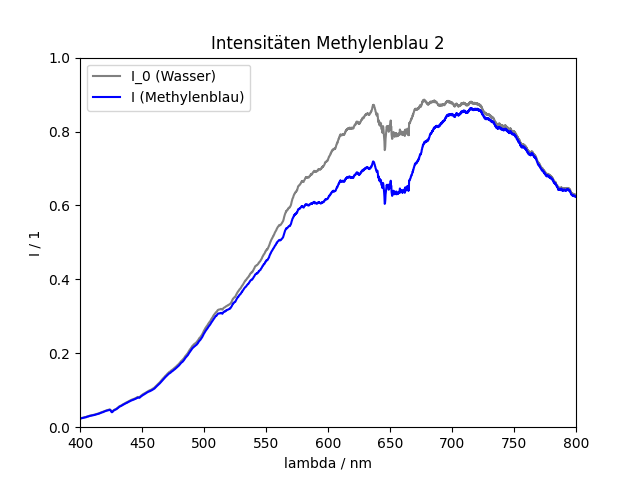
\includegraphics[scale=0.6]{MB_Intensitaeten_2.png}
%\end{figure}





\subsection{Bestimmung der Dicke einer Glasplatte durch das Transmissionsspektrum}

Zur Bestimmung der Dicke einer Glasplatte wird zuerst ein Referenzspektrum gemessen und danach die Glasplatte in den Strahlengang eingesetzt. Die Intensität von Glasplatte und das dazugehörige Referenzspektrum ist in Grafik~\ref{fig:I_glas_1} dargestellt.


\begin{figure}[H]
\centering
\caption{Zusammenhang zwischen Intensität und Wellenlänge von Glasplatte 1 und ein gemessenes Referenzspektrum. Es wird Probe 1 aus der Angabe verwendet.}
\label{fig:I_glas_1}
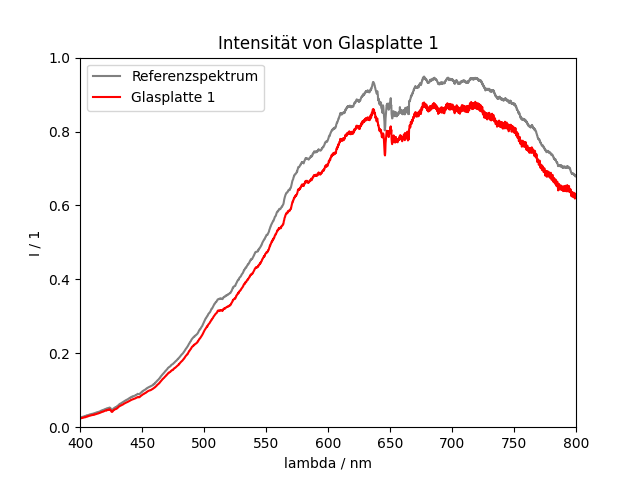
\includegraphics[scale=0.7]{GP_Intensitaet_1.png}
\end{figure}



%\begin{figure}[H]
%\centering
%\caption{Zusammenhang zwischen Intensität und Wellenlänge von Glasplatte 2 und ein gemessenes Referenzspektrum.}
%\label{fig:I_glas_2}
%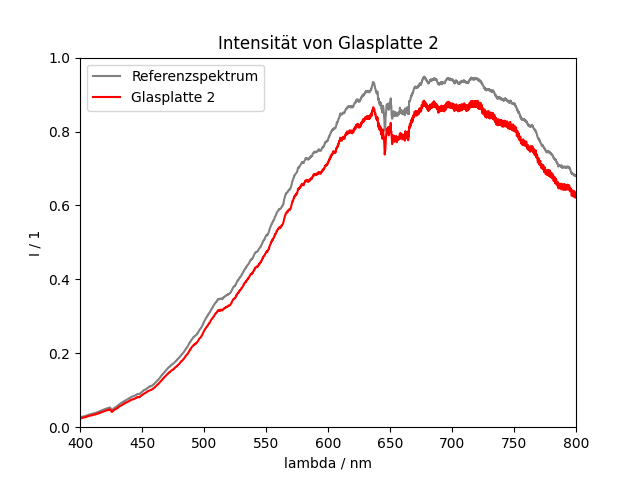
\includegraphics[scale=0.7]{GP_Intensitaet_2.png}
%\end{figure}



\section{Auswertung}

\subsection{Bestimmung von Transmission und Extinktion für verschiedene Farbfilter}

Die Transmissionen und die Extinktionen der Filter bzw. Filterkombinationen werden durch die Formeln \eqref{eq:trans} und \eqref{eq:ex} bestimmt. Die Transmissionen sind in Grafik~\ref{fig:T_Farben} und die Extinktionen in Grafik~\ref{fig:Ext} zusammengefasst.

In Grafik~\ref{fig:sum_ext_1} wurde zusätzlich grafisch gezeigt, dass die Extinktion vom blauen und roten Filter in Summe jene Extinktion ergibt, welche bei der Kombination aus den beiden Filtern gemessen wurde. Damit wurde die Additivität experimentell gezeigt. Nach den Regeln für Logarithmen muss auch die Multiplikation der Transmissionen erfüllt sein. Das wurde in Grafik~\ref{fig:mult_trans_1}




\begin{figure}[H]
\centering
\caption{Zusammenhang zwischen Transmissionen und Wellenlänge bei gegebenen Filter.}
\label{fig:T_Farben}
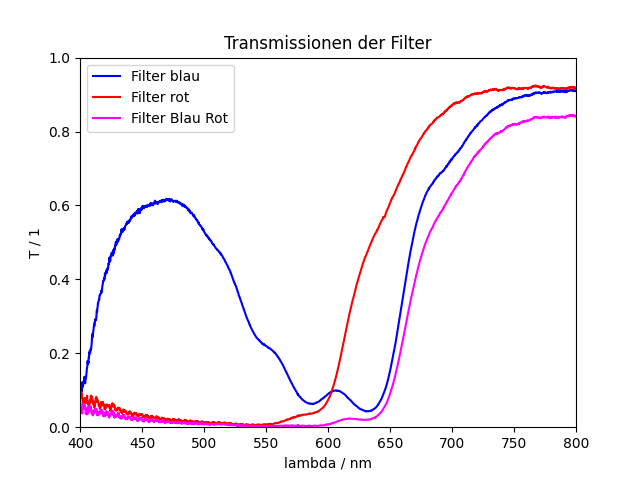
\includegraphics[scale=0.6]{FF_Transmissionen.png}
\end{figure}



\begin{figure}[H]
\centering
\caption{Zusammenhang zwischen Extinktion und Wellenlänge bei gegebenen Filter.}
\label{fig:Ext}
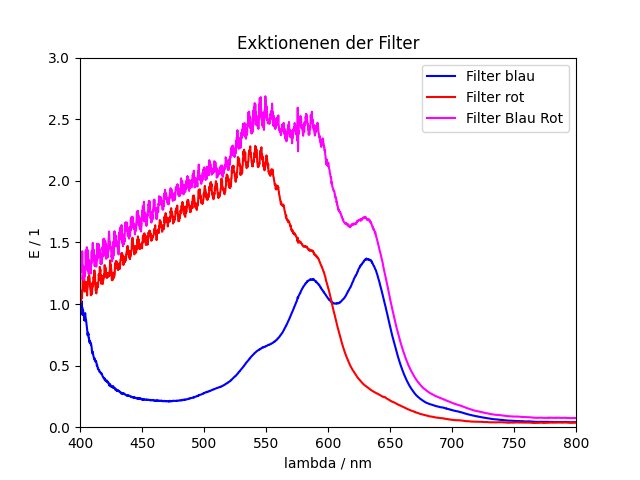
\includegraphics[scale=0.6]{FF_Extinktionen.png}
\end{figure}

\begin{figure}[H]
\centering
\caption{Summe der Extinktionen des roten und blauen Filters (jeweils extra gemessen) hier in grau verglichen mit der gemeinsam gemessenen Extinktion hier in magenta.}
\label{fig:sum_ext_1}
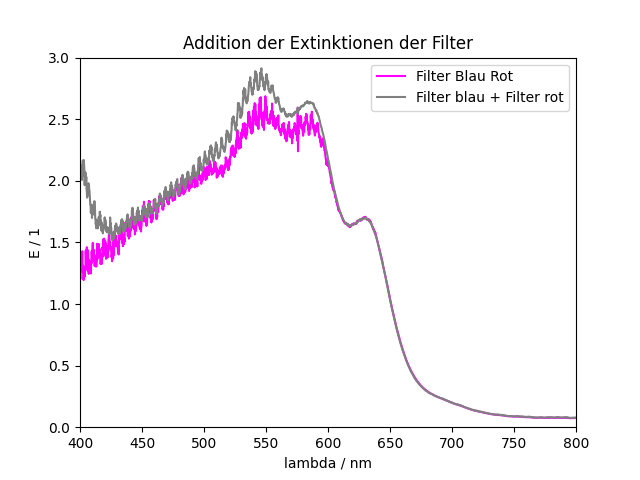
\includegraphics[scale=0.6]{FF_Extinktionen_addition_1.png}
\end{figure}




\begin{figure}[H]
\centering
\caption{Produkt der Transmissionen des roten und blauen Filters (jeweils extra gemessen) hier in grau verglichen mit der gemeinsam gemessenen Transmission hier in magenta.}
\label{fig:mult_trans_1}
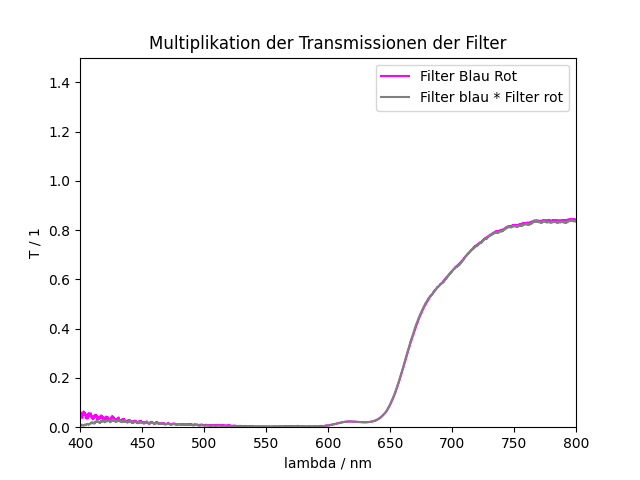
\includegraphics[scale=0.6]{FF_Extinktionen_multiplikation_1.png}
\end{figure}





%\begin{figure}[H]
%\centering
%\caption{Summe der Extinktionen des gelben und blauen Filters (jeweils extra gemessen) hier in grau verglichen mit der gemeinsam gemessenen Extinktion hier in grün.}
%\label{fig:sum_ext_2}
%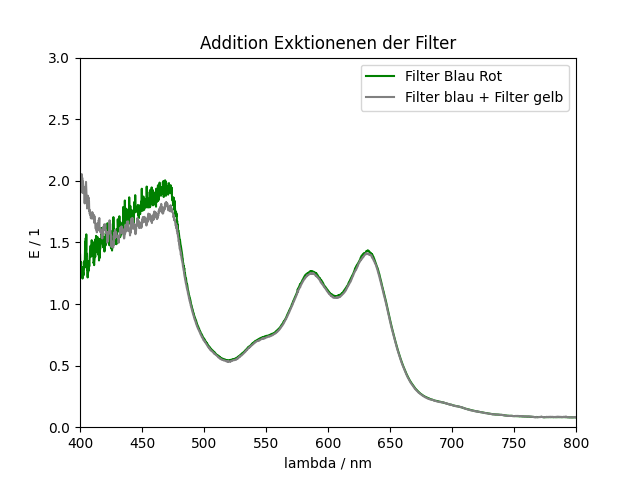
\includegraphics[scale=0.7]{FF_Extinktionen_addition_2.png}
%\end{figure}

%
%
%\begin{figure}[H]
%\centering
%\caption{Intensitäten bei Vertauschung der Reihenfolge der Filter. Es ist kaum ein Unterschied zu erkennen. Daher ist in Grafik \ref{fig:reihenfolge2} die Differenz dargestellt.}
%\label{fig:reihenfolge1}
%
%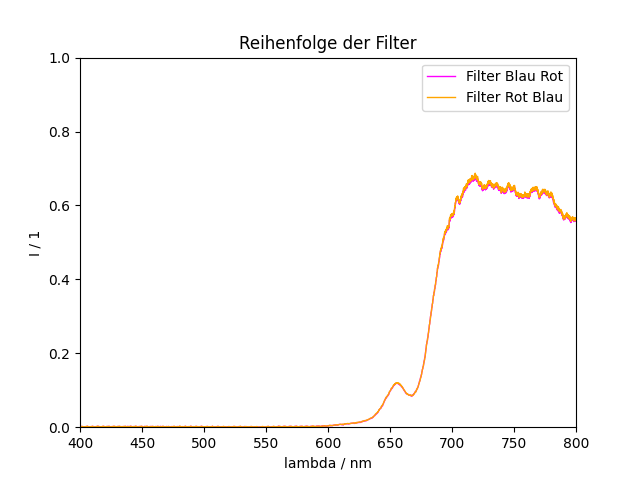
\includegraphics[scale=0.7]{reihenfolge1.png}
%\end{figure}
%
%
%
%\begin{figure}[H]
%\centering
%\caption{Differenz der Intensitäten bei Vertauschung der Reihenfolge der Filter. Man kann hier eine Unsicherheit für die Auswertung ablesen.}
%\label{fig:reihenfolge2}
%
%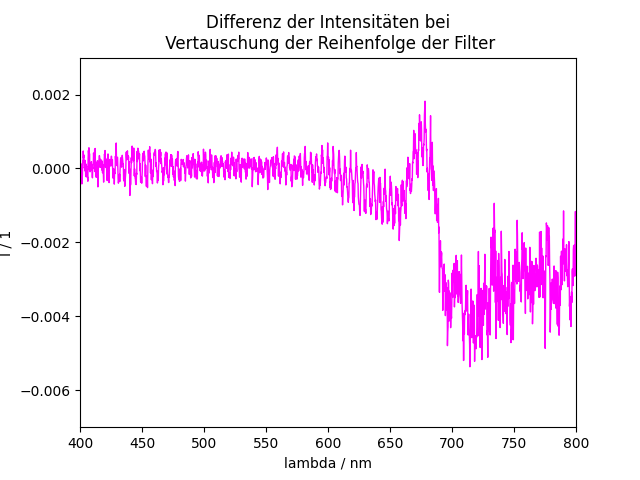
\includegraphics[scale=0.7]{reihenfolge2.png}
%\end{figure}






\subsection{Bestimmung der Stoffmengenkonzentration einer Methylenblaulösung}

Grafik~\ref{fig:MB_ET_1} zeigt die Transmission und Extinktion der Lösung. Für die Messung wurde Probe 1 der Aufgabenstellung verwendet.

Zur Berechnung der Konzentration benötigt man Formel~\eqref{eq:konzentration}. Durch Umformungen, Regeln für Logarithmen und Fehlerrechnung erhält man
\begin{align*}
c = \frac{\log(I_0) - \log(I_T)}{\varepsilon\cdot d} \pm \left(\frac{\dfrac{\Delta I_0}{I_0} + \dfrac{\Delta I_T}{I_T}}{\varepsilon\cdot d} + \frac{\log(I_0) - \log(I_T)}{\varepsilon\cdot d^2} \cdot \Delta d\right)
\end{align*}
Der Term $E = \log(I_0) - \log(I_T)$ kann aus den Grafiken abgelesen werden oder auch direkt durch die gemessenen Intensitäten berechnet werden.
Gemäß \cite{moodle} können wir den  dekadischer Extinktionskoeffizienten von Methylenblau bei einer Wellenlänge von 664~nm bei
\begin{align*}
\varepsilon =  77790~\frac{\text{Liter}}{\text{mol~cm}}
\end{align*}
annehmen. Die Schichtdicke der Lösung in der Küvette beträgt außerdem 1~cm mit der angenommenen Unsicherheit von $10~\mu$m. Insgesamt ergibt sich 
\begin{align*}
c_1 &= (2.04 \pm 0.08)\cdot 10^{-6}~\text{mol/Liter}  
\end{align*}

wobei die Werte für $I_0$ und $I_T$ mit Hilfe eines Python Skriptes gemittelt wurden.

\begin{figure}[H]
\centering
\caption{Transmission und Extinktion der Lösung mit Methylenblau 1.}
\label{fig:MB_ET_1}
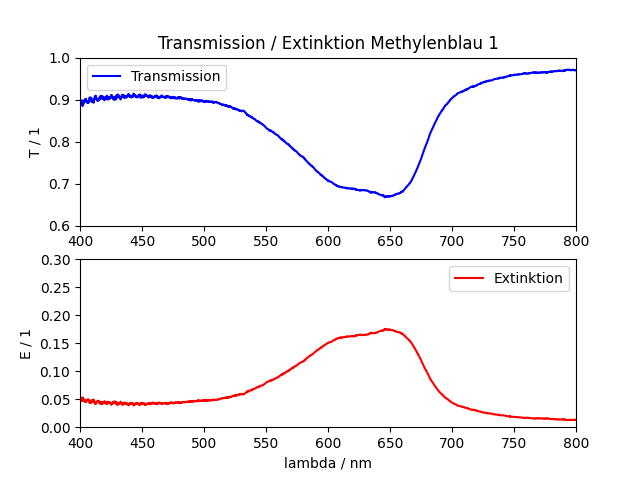
\includegraphics[scale=0.7]{MB_ET_1.png}
\end{figure}

%\begin{figure}[H]
%\centering
%\caption{Transmission und Extinktion der Lösung mit Methylenblau 2.}
%\label{fig:MB_ET_2}
%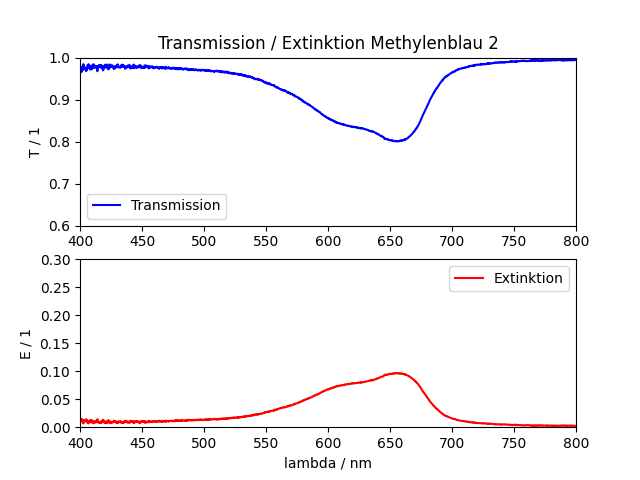
\includegraphics[scale=0.7]{MB_ET_2.png}
%\end{figure}




\subsection{Bestimmung der Dicke einer Glasplatte durch das Transmissionsspektrum}

Die Maxima der Intensität aus Grafik~\ref{fig:I_glas_1} ist gegeben durch
\begin{align*}
I_{1,\text{max}} &= 0.88\qquad \text{bei} \qquad \lambda_1 = 718.74 
\end{align*}

In Grafik~\ref{fig:GP1_ET} wird die Skalierungen so gewählt, dass der Bereich zwischen 700 und 720~nm genauer betrachtet werden kann. Dort werden die Maxima der Transmission abgelesen. Diese sind in Tabelle~\ref{tab:GP_max_glas1} zusammengefasst.

\begin{table}[H]
\centering
\caption{Transmissionsmaxima im Bereich $\lambda_m\in[700,720]~$nm. $m$ Begungsordnung, $\nu_m$ Wellenzahl, $T_{1,m}$ Wert der Transmission von Platte 1 gemäß Angabe.}
\label{tab:GP_max_glas1}
\begin{tabular}{cccc}
m & $\lambda_m$ / nm & $\nu_m$ / $\mu$m${}^{-1}$ & $T_{1,m}$ / 1 \\
\hline1 & 700.5 & 1.428 & 0.928\\
2 & 701.7 & 1.425 & 0.927\\
3 & 702.6 & 1.423 & 0.929\\
4 & 703.8 & 1.421 & 0.928\\
5 & 704.7 & 1.419 & 0.929\\
6 & 705.9 & 1.417 & 0.928\\
7 & 706.8 & 1.415 & 0.930\\
8 & 708.0 & 1.412 & 0.931\\
9 & 708.9 & 1.411 & 0.929\\
10 & 710.1 & 1.408 & 0.929\\
11 & 711.3 & 1.406 & 0.929\\
12 & 712.2 & 1.404 & 0.930\\
13 & 713.4 & 1.402 & 0.931\\
14 & 714.5 & 1.400 & 0.929\\
15 & 715.5 & 1.398 & 0.931\\
16 & 716.6 & 1.395 & 0.930\\
17 & 717.8 & 1.393 & 0.929\\
18 & 718.7 & 1.391 & 0.931\\
19 & 719.9 & 1.389 & 0.931\\
\end{tabular}

\end{table}


%\begin{table}[H]
%\centering
%\caption{Transmissionsmaxima im Bereich $\lambda_m\in[700,720]~$nm. $m$ Begungsordnung, $\nu_m$ Wellenzahl, $T_{2,m}$ Wert der Transmission von Platte 2}
%\label{tab:GP_max_glas2}
%\begin{tabular}{cccc}
m & $\lambda_m$ / nm & $\nu_m$ / $\mu$m${}^{-1}$ & $T_{2,m}$ / 1 \\
\hline1 & 700.3 & 1.428 & 0.932\\
2 & 701.4 & 1.426 & 0.933\\
3 & 702.4 & 1.424 & 0.933\\
4 & 703.5 & 1.421 & 0.933\\
5 & 704.5 & 1.419 & 0.934\\
6 & 705.6 & 1.417 & 0.934\\
7 & 706.6 & 1.415 & 0.933\\
8 & 707.8 & 1.413 & 0.935\\
9 & 708.7 & 1.411 & 0.934\\
10 & 709.9 & 1.409 & 0.935\\
11 & 711.0 & 1.406 & 0.935\\
12 & 712.0 & 1.405 & 0.934\\
13 & 713.1 & 1.402 & 0.934\\
14 & 714.1 & 1.400 & 0.933\\
15 & 715.2 & 1.398 & 0.937\\
16 & 716.4 & 1.396 & 0.934\\
17 & 717.3 & 1.394 & 0.934\\
18 & 718.5 & 1.392 & 0.937\\
19 & 719.4 & 1.390 & 0.935\\
\end{tabular}

%\end{table}

Aus \cite{moodle} geht hervor, dass die Brechzahl bei Glas $n_p = 1.519$ ist, wenn $\lambda=700~$nm. Wir nehmen zusätzlich $\Delta n_p = 0.001$ an.
Zusätzlich besteht laut \cite{moodle} ein linearer Zusammenhang 
\begin{align*}
\nu_M = k\cdot m
\end{align*}
Durch Lineare Regression lässt sich dieses $k$ berechnen. Zusätzlich gilt
\begin{align*}
k = \frac{1}{2\cdot n_p\cdot d}
\end{align*}
wobei $d$ unsere gesuchte Dicke ist. Durch Berechnung der Regression ergibt sich
\begin{align*}
k_1 &= (-2.13 \pm 0.08)\cdot 10^{-6}~\text{nm}^{-1} 
\end{align*}

und daraus folgt
\begin{align*}
d = \frac{1}{2\cdot n_p\cdot k} \pm \left( \frac{\Delta n_p}{2\cdot n_p^2\cdot k} + \frac{\Delta k}{2\cdot n_p\cdot k^2}\right)
\end{align*}


Die Regression kann grafisch verdeutlicht werden
\begin{figure}[H]
\centering
\caption{Regression: Zusammenhang zwischen Maxima und Wellenzahl. Auf der x-Achse ist jeweils die Ordnung des Maximums aufgetragen, während auf der y-Achse die Wellenzahl in der Einheit $\mu$m$^-1$ aufgetragen ist.}
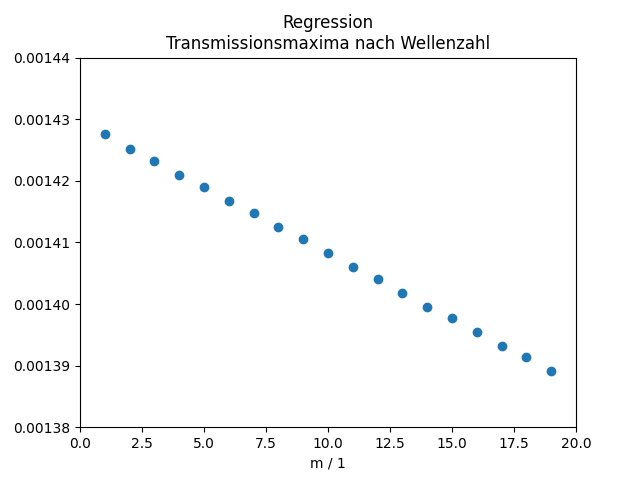
\includegraphics[scale=.5]{GP1_scatterplot_2.png}
\end{figure}


Die Dicke der Glasplatte beträgt letztendlich
\begin{align*}
d_1 &= (0.15 \pm 0.01)~\text{mm} 
\end{align*}


\begin{figure}[H]
\centering
\caption{Transmission und Extinktion bei Untersuchung von Glasplatte 1. Die Maxima der Transmission sind mit einer vertikalen Linie gekennzeichnet.}
\label{fig:GP1_ET}
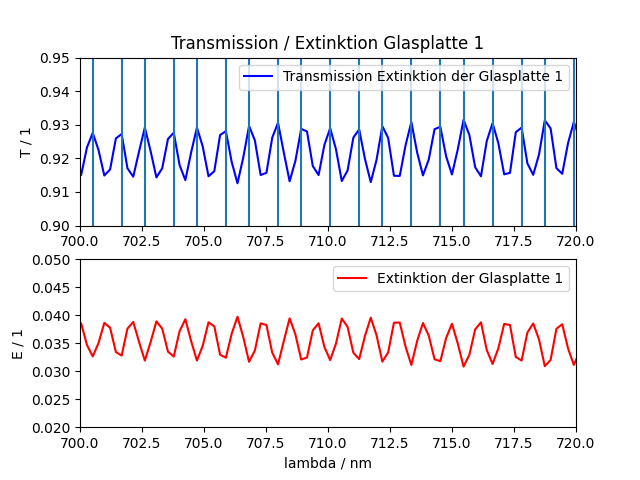
\includegraphics[scale=0.7]{GP1_ET.png}
\end{figure}


%\begin{figure}[H]
%\centering
%\caption{Transmission und Extinktion bei Untersuchung von Glasplatte 2. Die Maxima der Transmission sind mit einer vertikalen Linie gekennzeichnet.}
%\label{fig:GP2_ET}
%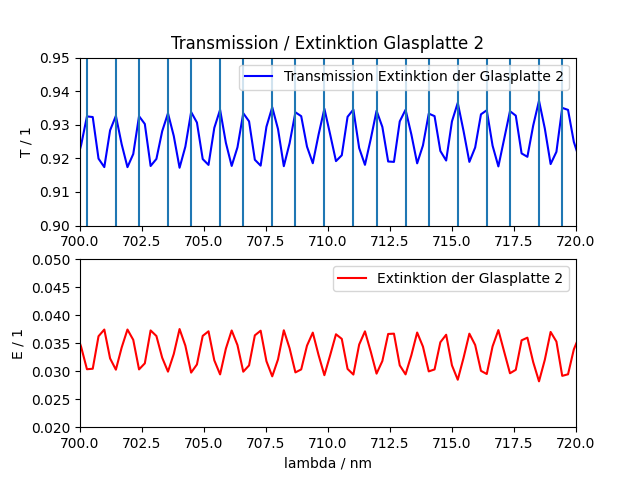
\includegraphics[scale=0.7]{GP2_ET.png}
%\end{figure}





\section{Diskussion}

Man kann in den aufgenommenen Spektren ein starkes Rauschen erkennen. Dies kann sich einerseits durch die Änderung von Lichtverhältnissen im Raum ergeben, andererseits durch leichte Unreiheiten auf den Linsen und Oberflächen der optischen Geräte.

%Die Reihenfolge der Farbfilter spielt eine untergeordnete Rolle. In Grafiken \ref{fig:reihenfolge1} und \ref{fig:reihenfolge2} kann man sehen, dass die Intensitäten sehr wenige Abweichungen haben.

Die Additivität von Extinktionen lässt sich auch mathematisch begründen. Sei $I_0$ die Intensität zu Beginn, $I_1$ nach Durchgang durch Filter 1 und $I_2$ die Intensität nach Durchgang durch Filter 2, dann gilt
\begin{align*}
E_1 + E_2 = \log\left(\frac{I_0}{I_1}\right) + \log\left(\frac{I_1}{I_2}\right) = \log\left(\frac{I_0}{I_1}\cdot \frac{I_1}{I_2}\right) = \log\left(\frac{I_0}{I_2}\right) = E_{1,2}
\end{align*}
Natürlich weicht die Summe in der Praxis durch das Rauschen etwas ab, aber insbesondere für Wellenlängen ab 600~nm ist eine sehr starke Übereinstimmung zu beobachten. Das Rauschen wird durch die Anwendung des Logarithmus verstärkt. Es ist mathematisch äquivalent die Multiplikativität der Transmissionen zu zeigen. Dies wurde in Grafik~\ref{fig:mult_trans_1} gemacht. Hier sieht man deutlich eine stärkere Übereinstimmung.

Natürlich gibt es weder für die Glasplatte, noch für die Methylenblau Lösung einen Literaturwert, da diese individuell sind.







\section{Zusammenfassung}

Es wurde die Transmission und die Extinktion eines blauen und roten Farbfilters (und deren Kombination) berechnet und veranschaulicht. Man erkennt leicht, dass die Transmission beim blauen Farbfilter zwischen 400~nm und 550~nm größer ist, da sich in diesem Bereich das blaue Farbspektrum befindet. Im Gegensatz dazu ist beim roten Filter die Transmission bei höheren Wellenlängen größer. Die Extinktionen sind bei Wellenlängen unter 600~nm stark rauschend, was wir auf die numerischen Eigenschaften der Logarithmusfunktion zurückführen. 

~

Zusätzlich war die Konzentration einer Methylenblaulösung zu bestimmen. Diese ist
\begin{align*}
c_1 &= (2.04 \pm 0.08)\cdot 10^{-6}~\text{mol/Liter}  
\end{align*}


Eine weitere Aufgabe war die Dicke einer gegebenen Glasplatte zu bestimmen.
\begin{align*}
d_1 &= (0.15 \pm 0.01)~\text{mm} 
\end{align*}



Die Ergebnisse bei den Farbfiltern stimmten mit unserem physikalischem Verständnis überein. Für die Dicke der Glasplatte und die Konzentration der Lösung gibt es klarerweise keine Vergleichswerte, da es sich um individuelle Eigenschaften der jeweiligen Probe handelt.




\begin{thebibliography}{9}
\bibitem{moodle} Unterlagen aus Moodle, J. Krenn, G. Paltauf, bereitgestellt von der KF Universität Graz.
\bibitem{demtroeder} W. Demtröder: \emph{Experimentalphysik 2 - Elektrizität  und Optik}, 7. Auflage, 2017.
\bibitem{monochromator} \url{https://de.wikipedia.org/wiki/Monochromator}, zugegriffen am 21.11.2020.
\end{thebibliography}


%\newpage 
%\appendix
%\section{Python Skript}



\definecolor{commentgreen}{RGB}{2,112,10}
\definecolor{eminence}{RGB}{108,48,130}
\definecolor{weborange}{RGB}{255,165,0}
\definecolor{frenchplum}{RGB}{129,20,83}

\lstdefinelanguage{python}{
    morekeywords={def, for, range, abs, return},
    otherkeywords={<-,->, |>, \%\{, \}, \{, \, (, )},
    sensitive=true,
    morecomment=[l]{\#},
    morecomment=[n]{/*}{*/},
    morecomment=[s][\color{purple}]{:}{\ },
    morestring=[s][\color{orange}]"",
    commentstyle=\color{commentgreen},
    keywordstyle=\color{eminence},
    stringstyle=\color{red},
	basicstyle=\ttfamily,
	breaklines,
	showstringspaces=false,
	frame=tb
}
\lstset{
extendedchars=\true,
inputencoding=utf8
}

%\lstinputlisting[language=Python,captionpos=b, label=lst:test,caption={Python Skript}]{plot.py}

%\lstinputlisting[language=Python,captionpos=b, label=lst:test,caption={Bessel Auswertung}]{generate_numbers_bessel.py}


%\lstinputlisting[language=Python,captionpos=b, label=lst:test,caption={Zerstreuungslinse Auswertung}]{generate_numbers_zerstreuungslinse.py}


\end{document}
